\documentclass[11pt]{article}

\usepackage[left=0.75in, right=0.75in, top=0.75in, bottom=0.75in]{geometry}
\usepackage{layout}
\usepackage{ucs}
\usepackage[utf8x]{inputenc}
\usepackage{titlesec}
\usepackage{graphicx}
\usepackage{amssymb}
\usepackage{amsmath}
\usepackage{dsfont}
\usepackage{float}
\usepackage{caption}
\usepackage{subcaption}
\usepackage{array}



\title{\textbf{TS113 - TP de communications numériques}}
\author{Maxime PETERLIN - Gabriel VERMEULEN\\\\{ENSEIRB-MATMECA, Bordeaux}}
\date{12 juin 2014}


\begin{document}

\maketitle
\tableofcontents

\newpage

\section{Communication numériques en bande de base}
	
	\subsection{Premier filtre de mise en forme}
		Dans cette partie, nous utiliserons le filtre de mise en forme suivant :
		\begin{equation}
			g(t) = 
			\left\{
		    	\begin{aligned}
		    		1&\,\,\,\,\,\, 0 \le t \textless T_s\\
		    		0&\,\,\,\,\,\, ailleurs
		      	\end{aligned}
		    \right.
		\end{equation}
		
		\subsubsection{Allure temporelle du signal $s_l(t)$}
			\begin{figure}[h]
				\centering
				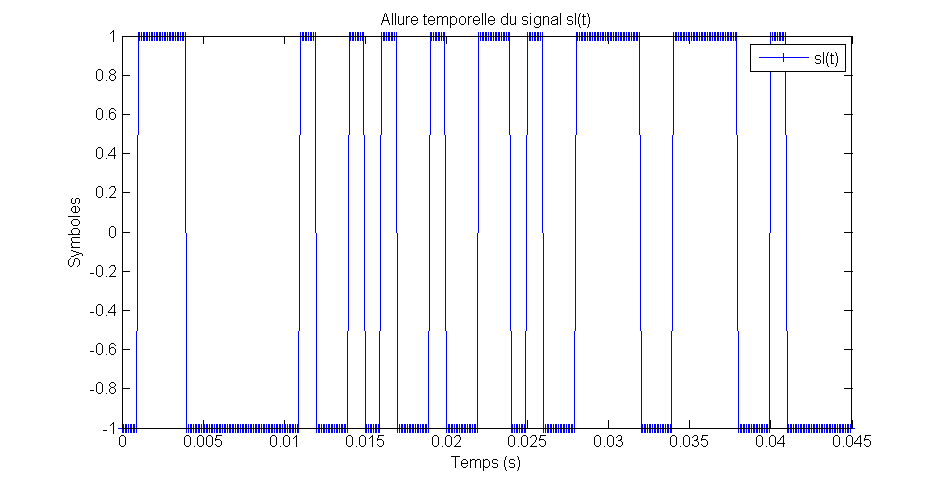
\includegraphics[scale=0.5]{images/Q311.png}
				\caption{Signal $s_l(t)$ pour $t \in [0, 50T_s-T_e]$}
				\label{Q311}
			\end{figure}
			$s_l$ est le signal en sortie du bloc correspondant à l'émetteur. \\
			La représentation temporelle de ce signal est directement liée au filtre de mise en fome où l'on retrouve le motif caractéristique de ce dernier.\\
			Cela se justifie notamment par la formule donnat $s_l$ : $s_l(t) = \sum\limits_{k \in \mathbb{Z}} A_kg(t-kT_s)$
			
		\subsubsection{Diagramme de l'oeil de $s_l(t)$}
			\begin{figure}[h]
				\centering
				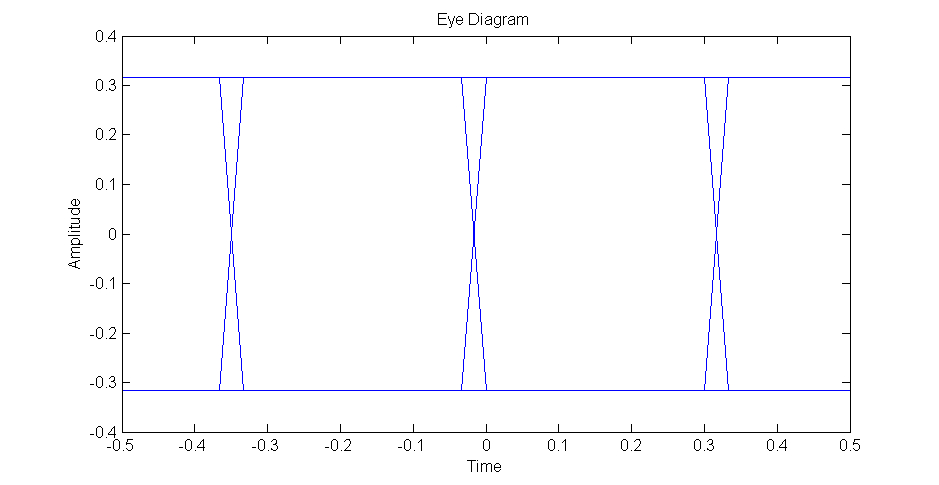
\includegraphics[scale=0.5]{images/Q312.png}
				\caption{Diagramme de l'oeil de $s_l(t)$ pour $3T_s$}
				\label{Q312}
			\end{figure}
			L'étude de la chaîne de communication se faisant sans bruit, il est normal de retrouver une ouverture de l'oeil qui soit maximale.\\
			De même l'ouverture horizontale est maximale, car l'échantillonneur n'induit pas de déphasage.
			
		\subsubsection{Allure temporelle du signal $r_l(t)$}
			\begin{figure}[h]
				\centering
				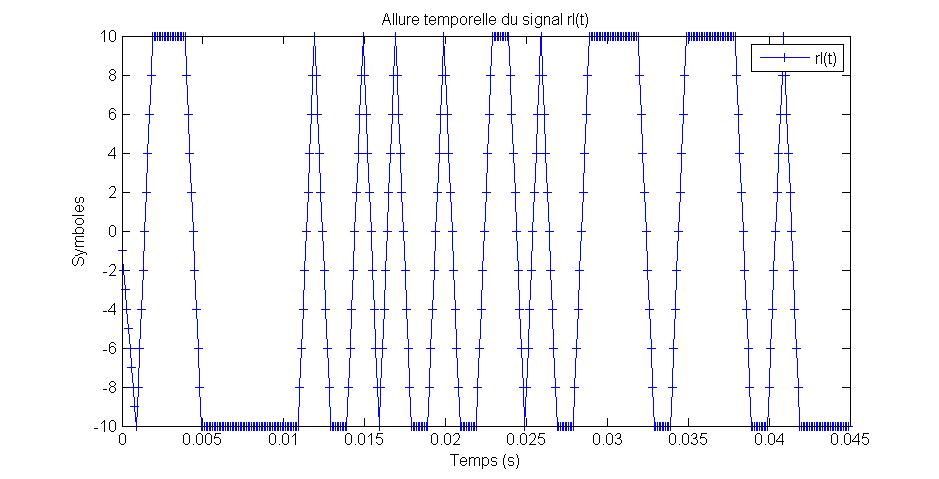
\includegraphics[scale=0.5]{images/Q313.png}
				\caption{Signal $r_l(t)$ pour $t \in [0, 50T_s-T_e]$}
				\label{Q313}
			\end{figure}
		
		
		\subsubsection{DSP de $s_l(t)$ et $s_s(t)$}
		\subsubsection{Évolution du TEB en fonction du rapport $\frac{E_b}{N_0}$}
		\subsubsection{Même manipulation avec une erreur de synchronisation temporelle}
		\subsubsection{Calcul de la perte de sensibilité du récepteur si le TEB $< 10^{-3}$}
	
	\subsection{Premier filtre de mise en forme}
		Dans cette partie, nous utiliserons le filtre de mise en forme suivant :
		\begin{equation}
			g_t(t) = 
			\left\{
		    	\begin{aligned}
		    		&(1-\frac{t}{T_s}) & \,\,\,\,\,\, 0 \le t \textless T_s\\
		    		&0 & \,\,\,\,\,\, ailleurs
		      	\end{aligned}
		    \right.
		\end{equation}
		
		\subsubsection{Allure temporelle du signal $s_l(t)$}
		\subsubsection{Diagramme de l'oeil de $s_l(t)$}
		\subsubsection{Allure temporelle du signal $r_l(t)$}
		\subsubsection{DSP de $s_l(t)$ et $s_s(t)$}
		\subsubsection{Évolution du TEB en fonction du rapport $\frac{E_b}{N_0}$}
		\subsubsection{Même manipulation avec une erreur de synchronisation temporelle}
		\subsubsection{Calcul de la perte de sensibilité du récepteur si le TEB $< 10^{-3}$}
		

\section{Communication numériques sur fréquence porteuse}
	\subsection{Étude théorique}
	\subsection{Étude expérimentale - Canal à bande passante infinie}


\end{document}
